\subsection{OB-7 (BEK)}
Základní bezpečnostní principy. Modelování bezpečnostních rizik, metodiky STRIDE a DREAD.

\begin{itemize}
    \item Hrozba --- potenciální příčina bezpečnostního incidentu
    \item Zranitelnost --- slabé místo aktiva/skupiny aktiv, které lze využít hrozbou/hrozbami
    \item bezpečný software --- chrání CIA (důvěrnost, integritu, dostupnost)
    \item spolehlivý software --- dělá jen to k čemu byl určen
    \item kvalitní software --- spolehlivý a bezpečný
    \item potřeba definovat bezpečnostní cíle pro aplikaci (kdo bude používat, co znamená pro uživatele bezpečnost, kde bude app provozována, co když...)
    \item secure by design --- bezpečnost se musí zahrnout již do návrhové fáze
    \item secure by default --- základní nastavení bude to nejvíce používané, musí být tedy bezpečné
    \item decure in deployment --- jak zařídit, aby aplikace byla bezpečná i po vydání (aktivní údržba, možnosti bezpečného nastavení)
    \item myslete jako útočník 
    \item minimalizujte plochu pro útok
    \item defense in depth --- víceúrovňová bezpečnost
    \item proncip nejnižších oprávnění
    \item zpětná kompatibilita je problém
    \item vstup je zlo
    \item plánujte selhání
\end{itemize}

\subsubsection*{Modelování hrozeb}
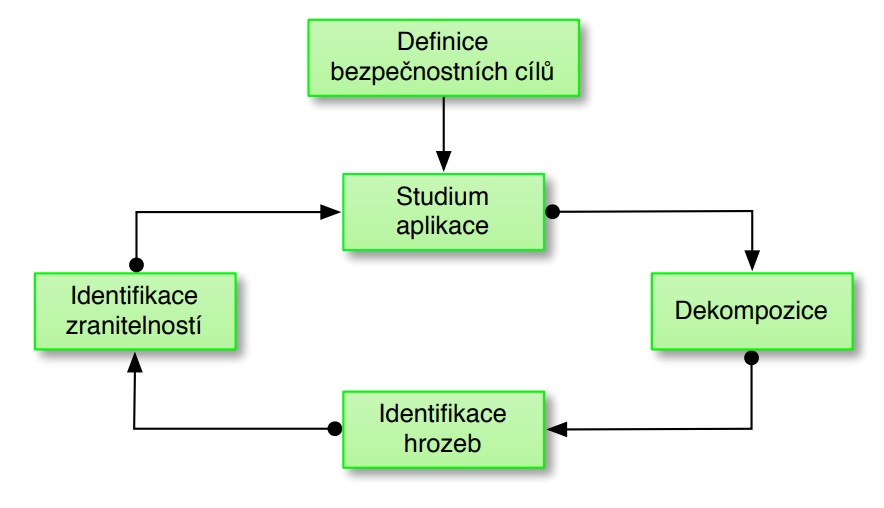
\includegraphics[width=0.6\textwidth]{img/OB-7_0.jpg}
\begin{itemize}

    \item Studium aplikace --- analýza designu aplikace s cílem určit komponenty, tok dat a hranice důvěry
    \item Dekompozice --- seskládání modelu z předchozích zjištění (z kroku 1), od vyšší úrovně níže, 2-3 opakování do hloubky
    \item Identifikace hrozeb --- popis komponent, uživatelů, administrátorů, autentizaci, .... a následně  pro každou komponentu zjišťovat, co může vzniknout za problémy, např. použít metodiku STRIDE --- výsledky zapsat do stromu / strukturovaného seznamu hrozeb --- každou hrozbu ohodnotíme, např podle metodiky DREAD
    \item identifikace zranitelností --- seřazení hrozeb dle skóre, vybereme ty které se reálně můžou stát, a použijeme jeden z následujících postupů:
    \begin{itemize}
        \item nechat hrozbu v programu
        \item informovat uživatele
        \item odstranit problém
        \item zmenšit/mitigovat hrozbu
    \end{itemize}
\end{itemize}

\subsubsection*{STRIDE}
\begin{itemize}
    \item Spoofing of Identity --- podvržení identity uživatele 
    \item Tampering with Data --- neautorizované pozměnění dat
    \item Repudiation --- popření transakce uživatelem 
    \item Information Disclosure --- únik informací
    \item Denial of Service --- odepření služby
    \item Elevation of Privilege --- neautrizované zvýšení oprávnění
\end{itemize}

\subsubsection*{DREAD}
\begin{itemize}
    \item Damage Potential --- potenciální rozsah způsobených škod
    \item Reproducibility --- jak snadné je hrozbu zopakovat
    \item Exploitability --- jak snadné je provedení útoku samotné
    \item Affected Users --- množství zasažených uživatelů
    \item Discoverability --- odhad obtížnosti nalezení
\end{itemize}